%%%%%%%%%%%%%%%%%%%%%%%%%%%%%%%%%%%%%%%%%%%%%%%%%%%%%%%%%%%%%%%%%%%%%%%%%%%%%%%%%%%%%%%%%%%%%%%%%%%%%%%%%%%%%%%%%%%%%%%%
\newpage
\chapter {\Large{Database Encryption}}
Data Secuirty plays important role when we talk about database. It protect your database from desctructive forces and the unwanted actions of unauthorized users.

\par
Android sqlite does not provide any protection against your database. There are many third party security implementation's which application developer can use in their application to protect their database.

\section{SQLCipher}
SQLCipher is an open source extension to SQLite that provides transparent 256-bit AES encryption of database file. SQLCipher has a small footprint and great performance so it's ideal for protecting embedded application databases and is well suited for mobile development.

\par
Siminov provide implementation for SQLCipher database encryption security. Its easy and secured to use it.

\par
Below are steps to make your application totally secured.

\begin{enumerate}

	\item \small Download SQLCipher from their website for android (\url{http://sqlcipher.net/downloads/}).

	\item \small Configure SQLCipher in your application. Follow below steps:

		\begin{enumerate}

			\newpage
			\item \small Copy \textbf{sqlcipher.jar}, \textbf{guava-r09.jar}, \textbf{commons-codec.jar} in your application libs folder.

				\begin{figure}[!htbp]
					\centering
						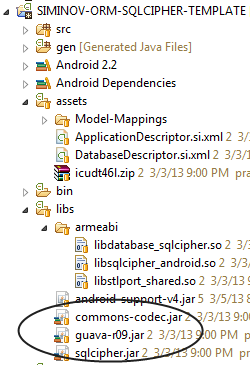
\includegraphics[height=8cm]{Resources/siminov_template_sqlcipher_application_setup_1.png}
					\end{figure}

			\item \small Copy dll file in your libs folder. 

				\begin{figure}[!htbp]
					\centering
						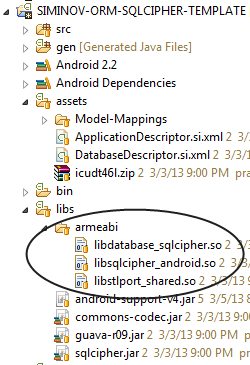
\includegraphics[height=8cm]{Resources/siminov_template_sqlcipher_application_setup_2.png}
					\end{figure}

		
			\newpage		
			\item \small Copy icudt461.zip in your application assets folder.

				\begin{figure}[!htbp]
					\centering
						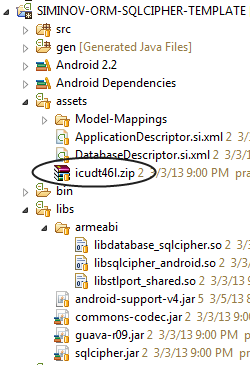
\includegraphics[height=8cm]{Resources/siminov_template_sqlcipher_application_setup_3.png}
					\end{figure}

		\end{enumerate}

		\par
		The stucture of your application should look like this.
	
				\begin{figure}[!htbp]
					\centering
						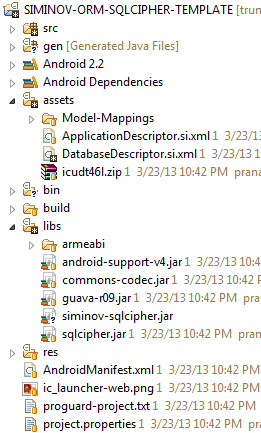
\includegraphics[height=8cm]{Resources/siminov_template_sqlcipher_application_setup.png}
					\end{figure}
	
	\newpage
	\item \small Download and copy Siminov SQLCipher jar in application libs folder.

				\begin{figure}[!htbp]
					\centering
						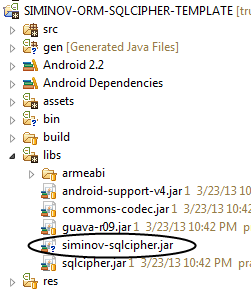
\includegraphics[height=7cm]{Resources/siminov_sqlcipher_template_application_add_siminov_sqlcipher_jar.png}
					\end{figure}

	\item \small To configure SQLCipher with Siminov add type property as sqlcipher and password attribute in DatabaseDescriptor.si.xml.

				\begin{figure}[!htbp]
					\centering
						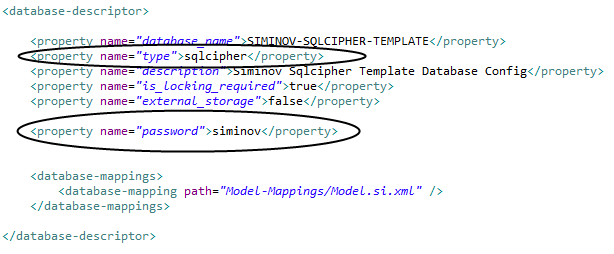
\includegraphics[height=4.3cm]{Resources/siminov_template_sqlcipher_application_sqlcipherdatabaseimpl_class_configure.png}
					\end{figure}

\end{enumerate}


					\begin{center}
						\colorbox{grey}{
						\parbox[t]{.8\linewidth}{
							\fontsize{11pt}{11pt}\selectfont % The first argument for fontsize is the font size of the text and the second is the line spacing - you may need to play with these for your particular title
							\vspace*{0.1cm} % Space between the start of the title and the top of the grey box
		
							\hfill \textbf{Note} \\
							For any future reference you can download SIMINOV-SQLCIPHER-TEMPLATE Application and can check how we have configured application with SQLCipher.
			

							\vspace*{0.0cm} % Space between the end of the title and the bottom of the grey box
						}
					}

					\end{center}
